\documentclass[tikz,border=5pt]{standalone}
\usepackage{amsmath}
\usetikzlibrary{arrows.meta,calc,decorations.pathreplacing}
\definecolor{ink}{HTML}{16324F}
\definecolor{teal}{HTML}{168A88}
\definecolor{gold}{HTML}{D9892B}
\definecolor{redq}{HTML}{B84A4A}
\definecolor{soft}{HTML}{EAF5F4}
\begin{document}
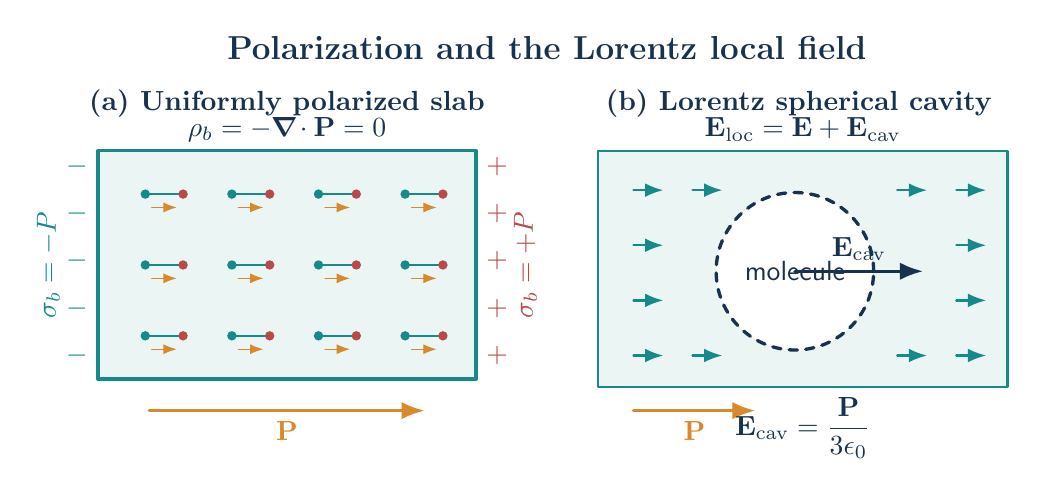
\begin{tikzpicture}[font=\sffamily,>=Latex,line cap=round,line join=round]
  \node[font=\bfseries\large,ink] at (6.15,4.85) {Polarization and the Lorentz local field};

  \begin{scope}[shift={(0,0)}]
    \node[font=\bfseries,ink] at (2.85,4.15) {(a) Uniformly polarized slab};
    \fill[soft] (.45,.65) rectangle (5.25,3.55);
    \draw[teal,very thick] (.45,.65) rectangle (5.25,3.55);
    \foreach \y in {.95,1.55,2.15,2.75,3.35}{
      \node[teal,font=\bfseries] at (.18,\y) {$-$};
      \node[redq,font=\bfseries] at (5.52,\y) {$+$};
    }
    \node[teal,rotate=90] at (-.18,2.1) {$\sigma_b=-P$};
    \node[redq,rotate=90] at (5.88,2.1) {$\sigma_b=+P$};
    \foreach \x in {1.05,2.15,3.25,4.35}{
      \foreach \y in {1.2,2.1,3.0}{
        \draw[teal,thick] (\x,\y)--++(.48,0);
        \fill[teal] (\x,\y) circle (1.7pt);
        \fill[redq] (\x+.48,\y) circle (1.7pt);
        \draw[->,gold] (\x+.08,\y-.17)--++(.32,0);
      }
    }
    \draw[->,gold,very thick] (1.1,.25)--(4.6,.25) node[midway,below] {$\mathbf P$};
    \node[ink] at (2.85,3.82) {$\rho_b=-\boldsymbol\nabla\!\cdot\mathbf P=0$};
  \end{scope}

  \begin{scope}[shift={(6.55,0)}]
    \node[font=\bfseries,ink] at (2.8,4.15) {(b) Lorentz spherical cavity};
    \fill[soft] (.25,.55) rectangle (5.45,3.55);
    \draw[teal,thick] (.25,.55) rectangle (5.45,3.55);
    \fill[white] (2.75,2.02) circle (1.0);
    \draw[ink,dashed,very thick] (2.75,2.02) circle (1.0);
    \node[ink] at (2.75,2.02) {molecule};
    \foreach \x/\y in {.7/.95,.7/1.65,.7/2.35,.7/3.05,1.45/.95,1.45/3.05,4.05/.95,4.05/3.05,4.8/.95,4.8/1.65,4.8/2.35,4.8/3.05}{
      \draw[->,teal,thick] (\x,\y)--++(.38,0);
    }
    \draw[->,gold,very thick] (.7,.25)--(2.25,.25) node[midway,below] {$\mathbf P$};
    \draw[->,ink,very thick] (2.75,2.02)--(4.38,2.02)
      node[midway,above] {$\mathbf E_{\rm cav}$};
    \node[ink,align=center] at (2.85,3.82)
      {$\displaystyle \mathbf E_{\rm loc}=\mathbf E+\mathbf E_{\rm cav}$};
    \node[ink,align=center] at (2.85,.03)
      {$\displaystyle \mathbf E_{\rm cav}=\frac{\mathbf P}{3\epsilon_0}$};
  \end{scope}
\end{tikzpicture}
\end{document}
